\chapter[Statistical Process Control]{Statistical Process Control}
\chaptermark{SPC}
\label{sec:spc}

Statistical process control (SPC), \aka \emph{change detection}, or \emph{novelty detection}, deals with the quantitative analysis of a ``process'', which may be a production line, a service, or any other repeated operation.\marginnote{Change Detection}
As such, SPC may be found in the Analyze, Improve, and Control stages of the DMAIC cycle.
The purpose of the SPC, in the terms coined by Shewhart, is to seperate the variability in the process into \emph{assignable} causes of variation and \emph{chance} causes of variation.\marginnote{Causes of variation}
Assignable are also known as \emph{special} causes, or simply \emph{signal}.
Chance causes are also known as \emph{common} causes of variation, or \emph{haphazard} variability, or simply \emph{noise}.
 
A process is said to be in \emph{statistical control} if all its variation is attributable to chance causes.
If this is not the case, we call it \emph{out of control} and we will seek the assignable causes, so that we may reduce variability by removing them.
All the statistical tools of chapters \ref{sec:exploratory} and \ref{sec:inference} may be called upon for this endeavour but in this chapter we focus on one particular such tool- the \emph{control chart}.
We start with the \emph{Shewhart control chart}, in which each value is charted using different data, from different periods. \marginnote{Shewhart Chart}



\section{The Run Chart}
The simplest possible control chart is the \emph{run chart}, in which each measured CTQ is simply plotted against the time of measurement.
If strong anomalies exist, or temporal patterns, they may be already visible in the run-chart.
On the down-side, the run-chart is essentially a statistical test to detect out-of-control behaviour based on a single observation at a time.
Knowledge of statistical hypothesis testing suggest we can do better. 
Enter the \barxChart. 


\section[The X-bar Chart]{The \barxChart}
\sectionmark{\barxChart}


We demonstrate the concepts and utility of control charts with the simplest, yet most popular of them all, the \barxChart. 
The chart borrows its name from the fact that it is essentially a visualization of the time evolution of the average ($\bar{x}$) of the CTQ. 
The chart is also augmented with visual aids that help in determining if the process is \emph{in control}, i.e., if it is consistent with its own history. 

\begin{remark}[Control Charts and Capability Analysis]
While seemingly very similar ideas, there is a fundamental difference between capability analysis and process control:  process control compares to the \emph{statistical regularity in the past}, while capability analysis compares to \emph{specification}.
Process capability and control charting ideas may be compounded, as we explain in Chapter~\ref{sec:advanced_capability_analysis}.
\end{remark}


An illustration of a \barxChart is given in Figure~\ref{fig:bar_x_chart}. 
The ingredients of this chart are the \emph{centerline} ($\mu_0$), lower and upper control limits (\emph{LCL, UCL}), and the statistic $\bar{x}_t$ evolving in time. 
If at each period $t$ we compute the average of the $n$ samples of the period. We denote $$\bar{x}_t:=\frac 1n \sum_{i=1}^n x_{it}.$$

\begin{figure}[ht]
\centering
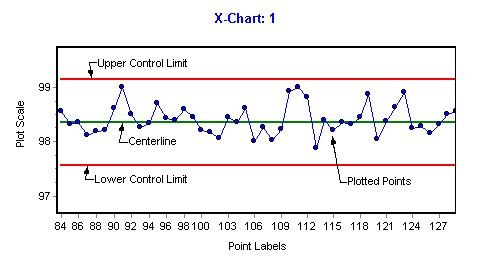
\includegraphics[height=0.3\textheight]{art/X-chartExample}
\caption[\barxChart]{\barxChart. \newline \url{https://mvpprograms.com/help/P-mvpstats/spc/WhatAreControlCharts}}
\label{fig:bar_x_chart}
\end{figure}

\paragraph{Phase I/II} 
Initially we assume the process it out of control, we identify and remove assignable causes of variation, until we are left with a ``well-behaved'' subset of data points, we believe to be in-control. 
We call this \emph{Phase I}, and we use it to initialize required quantities such as the centre line $(\hat{\mu}_0)$ and stadard errors $\sigma_{\bar{x}}$. 
After the chart has been calibrated, and major assignable sources of variability removed, we can finally start monitoring the process, known as \emph{Phase II}.


Figure~\ref{fig:bar_x_chart} makes it evident \barxChart requires us to make several design decisions.
A standard design decision is setting the centerline as average of a subset of $\tau$ periods that we believe to be in control. Phase I may provide us with such a sample.
\begin{align}
\label{eq:centerline}
	\hat{\mu}_0=\frac 1\tau \sum_{t=1}^\tau \bar{x}_t,
\end{align}
where $\mu_0$ denotes the in-control expectation of the process, and summation is over the $\tau$ in Phase I we believe to be in control.
Notation originates from treating the in-control process as a null hypothesis, as it should be thought of.

\bigskip

Back to the design decisions we make when designing a control chart.
\begin{tcolorbox}[breakable]
\paragraph{Design decisions}
\begin{enumerate}
\item Centerline ($\mu_0$).
\item Upper and lower confidence limits: UCL and LCL (do not confuse with USL and LSL!).
\item Sample size in each sample, denoted $n$.
\item The within period sampling scheme, known as \emph{rational groupings}.
\item The between-period sampling scheme, notably the \emph{frequency of samples}, denoted $h$. 
\item Other stopping rules.
\end{enumerate}
\end{tcolorbox}

These design decisions ultimately govern the error rates of the chart, which in turn, incur financial costs. 
For now we will restrict attention to type I/II error rates, until Section~\ref{sec:economical_considerations} where we consider these choices as an economical optimization problem.

For ease of exposition, control chart design is demonstrated for the \barxChart, but equally applies to other control charts, presented in Section~\ref{sec:other_control_charts}.

We start by a type I error rate analysis. 
Denote $\alpha_t$ the false alarm probability at period $t$.
How do our design choices affect $\alpha_t$?
\begin{align}
	\alpha_t &:= 1-P_{H_0}(\bar{x}_t \in [LCL,UCL]) \\
	&= 2 P_{H_0}(\bar{x}_t < LCL) \\
	&= 2 P_{H_0}(Z<\frac{LCL-\mu}{\sigma_{\bar{x}}}) \\
	&= 2 P_{H_0}(Z < -\arm) \\
	&= 2 \Phi(-L)
\end{align}
The above follows from choosing $UCL:=\mu_0 + \arm \sigmabar, LCL:= \mu_0 - \arm \sigmabar$, $\x_{it}\sim \gauss{\mu,\sigma^2}$, and $\sigmabar$ being the standard deviation of the statistic being monitored, which we can estimate, for example, from Phase I. 
For instance: 
$\widehat{\sigmabar^2}=\frac{1}{\tau-1} \sum_t^\tau (\bar{x}_t- \hat{\mu_0})^2 $
In this case, $\sigmabar=\frac{\sigma_x}{\sqrt{n}}$.
A typical design choice is $\arm=3$, known as \emph{3-sigma control limits}, implying a false alarm rate of $\alpha_t=0.0027$.\marginnote{3-Sigma Control Limits}
Since we assumed the process is fixed over time, then so is $\alpha_t$ and we can simply write $\alpha_t=\alpha$.

A power analysis for our design choices follows the same lines.
Denote by $H_1$ the out-of-control distribution,  $\beta_t$ the type-II error rate, and $\pi_t=1-\beta_t$ the power, at period $t$.
We then have
\begin{align}
	\pi_t &:= 1-P_{H_1}(\bar{x}_t \in [LCL,UCL])
\end{align}
and the rest follow from the distribution of $\bar{x}_t$ when the process is out of control.
Since the out-of-control shift is (asumingly) stable, we can again omit the time index and write $\pi=\pi_t$.
Assuming the out-of-control process is a shift of magnitude $k \sigma$, i.e.: 
$\x \sim_{H_1} \gauss{\mu_1,\sigma^2}; \mu_1=\mu_0+ k \sigmabar$, we plot in Figure~\ref{fig:power_function}, the detection power of a 3-sigma \barxChart as a function of $k$. 
This is known in the statistical literature as a \emph{power function}, and in the engineering literature as the \emph{operator characteristic} (OC).\marginnote{Operator Characteristic}


\begin{figure}[h]
\centering
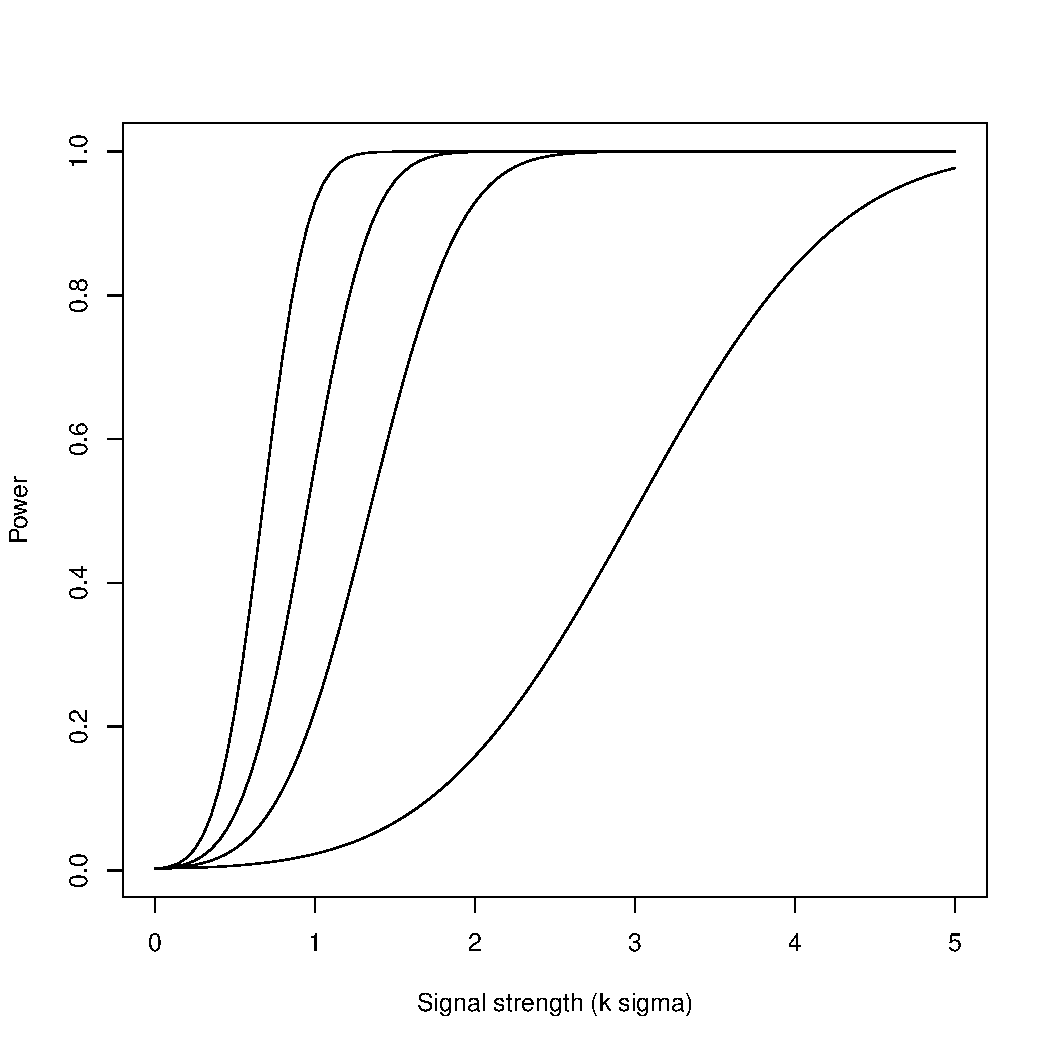
\includegraphics[height=0.3\textheight]{art/power_function.pdf}
\caption[Power Function]{
\footnotesize
Power function of the 3-sigma \barxChart with $n=5,10,20$ and $\mu_1=\mu_0 + k \sigma$.}
\label{fig:power_function}
\end{figure}

\begin{remark}[3-Sigma rule]
At the risk of stating the obvious, the ``sigma'' in the 3-Sigma rule will always be that of the statistic being monitored.
If we are monitoring $\bar{x}_t$, we will use $\pm 3 \sigmabar$. 
In particular, if $n=1$, then obviously $\sigmabar=\sigma_x$. 
More generally, if we are monitoring some $T(x)_t$, we will use $\pm 3 \sqrt{\var{T(x)_t}}$.
\end{remark}

\begin{remark}[3-Sigma Control Limits vs. 3-Sigma Capability]
Do not confuse these two similar ideas.
3-Sigma Control Limits is a statement on the false alarm rate. It tells you nothing on the probability of non-compliance. 
3-Sigma Capability is a statement on the probability of a unit to be defect. 
Monitoring production via its capability is very rare, as we would like the alarms to sounds long before defect units leave the production line.
\end{remark}



\begin{extra}[Operator Characteristics]
Many operator characteristics have been proposed to study the performance of control charts, statistical tests, or binary classifiers in general.
You may be already familiar with some, such as the Reciever Operator Charachteristic (ROC). 
The curious reader is referred to \cite{wikipedia_receiver_2015} for more information.
\end{extra}


A very important quantity is the \emph{average run length} (ARL), which is the expected number of periods between two crossings of control limits, i.e., the expected periods between alarms. \marginnote{ARL}
We denote by $ARL_0$ the ARL when the process is under statistical control, and $ARL_1$ otherwise\footnote{Note that it is implied that the process has a \emph{stable} distribution, even though it is out if control.}. 
For Shewhart charts, where $\bar{x}_t$ are statistically independent and $\alpha_t,\pi_t$ fixed in time, then clearly the number of periods until a crossing is geometrically distributed. Using the expectation of a geometric random variable we can conclude that 
\begin{align}
	ARL_0=1/\alpha \label{eq:arl_0}, \\
	ARL_1=1/\pi \label{eq:arl_1}.
\end{align}
ARL is measured in periods. 
We can convert to time units by multiplying the ARL by the duration of sampling interval ($h$).
This is known as the \emph{average time to signal} (ATS).\marginnote{ATS}
It is quite common to design a control chart so that it achieves a particular $ATS_0$.

\begin{remark}[ARL more important than type-I error]
In the case of Shewhart charts, there is a simple mapping between ARL and type I error rates.
This need not be the case for general control charts. 
Since type I errors will occur with certainty if the process runs long enough, then it is actually the ARL that is more informative than type-I errors when designing a control chart.
\end{remark}


Now assume that we are unhappy with our control chart. 
It simply makes too many false alarms, or takes too long to detect loss of statistical control.
What can we do about it?
Well, this is exactly the same question as when increasing the power or lowering the type I error of a statistical hypothesis test. This is obviously no coincidence, since control charts are nothing but a statistical test!
Here are some action courses:
\begin{enumerate}
\item Increase $\arm$. This is the same as shrinking the rejection region: 
it will decrease the false alarm rate, at the cost of power.
\item Increase $n$. Brilliant! Statistically, there is nothing to lose. It may, however, cost time and money.
\item Increase the sampling frequency $h$. Brilliant again! Nothing to lose, except time and money.
\item Change the sampling scheme within period. We elaborate on this in Section~\ref{sec:rational_grouping}.
\item Add other stopping rules: 
this acts just like growing the rejection region. It will increase power, at the cost of type I error. 
We elaborate in Section~\ref{sec:stopping_rules}.
\item Pool together more periods. See Section~\ref{sec:running_windows}.
\item Measure many CTQs simultaneously. See Section~\ref{sec:multivariate}. 
\end{enumerate}






\subsection{Control Limits and the Alarm Rate}
Ceteris paribus, $\arm$ governs the tradeoff between type I and type II errors, or sensitivity versus specificity.
It is very common to set $\arm=3$. 
For a normally distributed CTQ, this implies $2,700$ false alarms per million periods. 
This also implies an $ARL_0$ of $1/\alpha \approx 370$ periods, which is conveniently, roughly one year if sampling once a day.
We may obviously, discard this $\arm=3$ convention, and directly set UCL and LCL so they guarantee some desirable false alarm rate, or ARLs.

\begin{extra}[Non Normal CTQ]
If normality of $\bar{x}_t$ can be assumed, then one may estimate $\mu_0$ and $\sigmabar$ from phase I, and set LCL and UCL by finding the $\arm$ that solves $2\Phi(-\arm)=\alpha$, for some desired $\alpha$. 
If normality cannot be assumed, there are many ways to go about. Here are some options:
\begin{enumerate}
\item If some other distribution can be assumed then problem solved.
We may compute the false alarm rate of particular limits either analytically, or computationally (by simulation).
\item Increase $n$: even if $\x_{it}$ is non normal, for large enough $n$, then $\bar{x}_t$ will be via the central limit theorem (CLT).
\item Use empirical quantiles: If phase I has returned enough data, then we may estimate 
$\x_{\alpha/2}$ and $\x_{1-\alpha/2}$ using the empirical quantiles of phase I. 
The false alarm rate will be $\alpha$ since $P(\x \not \in [\hat{\x}_{\alpha/2},\hat{\x}_{1-\alpha/2}]) \approx \alpha$.
This is a \textbf{super practical} way to go about. The only downside of this avenue, is that you do not always have enough in-control data from phase I.
\end{enumerate}

\end{extra}



\subsection{Rational Groupings}
\label{sec:rational_grouping}

Recall that at each period we compute the average of $n$ samples. 
To fix ideas, think of a period being a day of production. 
How should we draw samples in this period? 
At the same time from the same machine?
At different times from the same machine?
Many configurations are possible, and the correct approach depends on the type of out-of-control behaviour one seeks. 
\emph{Rational groupings} merely reminds us to sample ``rationally'' in each period. 
Quoting \cite{montgomery_introduction_2007}'s words of caution:
\begin{quotation}
\dots we can often make any process appear to be in statistical control just by stretching out the interval between observations in the sample.
\end{quotation}






\subsection{Other Stopping Rules}
\label{sec:stopping_rules}

The assumption that we may only create alarms if $\bar{x}$ exceeds some control limits is needlessly restrictive.
A first relaxation is by allowing multiple regions.
It is quite common to define \emph{warning limits} and \emph{action limits}. Each may have its own alarm rate.
We may even change the sapling scheme if limits are breached. Increasing the sampling rate once the warning limits have been breached is known as \emph{adaptive sampling}, or \emph{variable sampling}, and it is a very efficient way to detect anomalies. \marginnote{Adaptive Sampling}
Another approach is to define multiple sets of stopping rules.
\begin{tcolorbox}[breakable]
\paragraph{WECO Rules}
\begin{enumerate}
\item One or more points\footnote{By ``point'' we mean the computed statistic at each period: $\bar{x}_t$.} outside of the 3-sigma control limits.
\item Two of three consecutive points outside the 2-sigma limits but still inside the 3-sigma control limits.
\item Four of five consecutive points beyond the 1-sigma limits.
\item A run of 8 consecutive points on one side of the centerline.
\end{enumerate}
\end{tcolorbox}

The above set of rules is known as the Western Electric Rules, \aka, the \emph{WECO} rules.\marginnote{WECO}
Augmenting the set of rules is the same as increasing a rejection region. It adds more sensitivity, at the cost of false alarms. If the rules are properly selected, the gain in sensitivity is worth the increase in false alarms.

As a quick exercise, we may compute $\alpha$  for $m$ independent rules, each with $\alpha^*$ type I error:
\begin{align}
\label{eq:multiplicity_in_spc}
	\alpha=1-(1-\alpha^*)^m.
\end{align}
Having 4 rules, like WECO, each at $\alpha^*=0.0027$ implies that we actually have $\alpha=0.01$ and $ARL_0 \approx 93$. For daily sampling of an in-control process, this means an alarm every quarter, and not every year. 
The good news is the analysis in Eq.(\ref{eq:multiplicity_in_spc}) does not apply to WECO, because the rules not independent but rather highly dependent. 
A can compute the $ARO_0$ of WECO in a quick simulation.

\begin{extra}[Stopping Rules]
There are many sets of stopping rules. 
These include WECO, Nelson, AIAG, Juran, Hughes, Duncan, Gitlow, Westgard, and more. 
See \url{http://www.quinn-curtis.com/spcnamedrulesets.htm} for a review.
\end{extra}







\section{Shewhart Charts With Other Test Statistics}

We have been focusing on the \barxChart for ease of exposition. There are, however, many cases where the mean is not an appropriate test statistic.
Examples include:
\begin{enumerate}
\item A discrete CTQ, where only the number of non-compliances can be counted. 
\item Where the departure from statistical control is not only a shift in $\mu$. 
\end{enumerate}

The following charts are designed for those cases. 
Practically all of the ideas presented for the \barxChart may be adapted to these other test statistics after appropriate adaptations. 
The reader is referred to \cite{montgomery_introduction_2007} for the details. 

\label{sec:other_control_charts}
\subsection{$R$ Chart}
Where $\bar{x}$ is replaced by the range, $\max_i\set{x_{it}}-\min_i\set{x_{it}}$.
This chart is sensitive to many changes in the distribution of the CTQ; the variance in particular. 
\subsection{$s$ Chart}
Where $\bar{x}$ is replaced by $s$. 
Sensitive to variability changes. 
This is an important and useful chart which we will revisit in Section~\ref{sec:multivarite_s}.
\subsection{$s^2$ Chart}
Like the $s$ chart, only in variance-scale.
\subsection{Regression Control Chart}
In a \emph{regression control chart}, the test statistic can be a regression coefficient. 
When compounded with multivariate charts, a regression control chart may accommodate several regression  coefficient, or the residuals. 
This is very useful if you allow the distribution of the CTQ to vary with some covariate, and you want to detect a change in this relation. 
To fix ideas, think that your CTQ depends on the temperature at the time of production. The distribution of the CTQ will thus vary with the temperature, but the break in their relation is cause for alarm.
\subsection{Derivative Chart}
If the break of control has occurred between periods (``the night shift guys broke it!''), the change in an \barxChart may carry more information (i.e., more power) than the value of $\bar{x}_t$ itself.
We can thus chart, not $\bar{x}_t$ itself, but rather, the \emph{change} in $\bar{x}_t$ between periods. 
It is quite possible $\bar{x}_t$ seems perfectly ok, but that $\bar{x}_t-\bar{x}_{t-1}$ seems highly irregular. 
Generalizing this idea, we can monitoring the \emph{derivative} of some statistic to detect this kinds of changes. 
\subsection{$p$ and $np$ Chart}
Where $\bar{x}$ is replaced by the proportion ($p$), or number ($np$), of non-conforming units.
Appropriate for attributes, i.e., categorical CTQs.
\subsection{$c$ Chart}
Like a $np$ chart, but where the number of nonconforming units is replaced with the total number of nonconformances, allowing multiple defects per unit. 
\subsection{$u$ Chart}
Like the $c$ chart, but allowing a variable number of units per period (varying $n$).





\section{Pooling Information Over Periods}
\sectionmark{Pooling Periods}
\label{sec:running_windows}

Assume an out-of-control process is a very mild shift of the mean controlled-process ($\mu$).
A power analysis may suggest that this shift is hard to detect, especially if $n$ is not too large (as seen in Figure~\ref{fig:power_function}).  
If the shift persists over periods, we may gain power, i.e., sensitivity, by pooling several periods together. 
We now present several ways to pool information from history. These are typically applied in Phase II, where out-of-control processes are expected to have only mild shifts, and not major ones as in Phase I. 

\begin{remark}[No longer Shewhart]
The name \emph{Shewhart control chart} is reserved to charts plotting one period at a time. 
When several periods are pooled together, we will no longer call this  ``Shewhart''.
\end{remark}

\begin{remark}[One observation at a time]
The following charts have a continuous flavour. As such, it is both favourable, and common, to compute them using one observation at a time, meaning that $n=1$. 
\end{remark}





\subsection{Moving Average Chart (MA)}
\sectionmark{MA}

One way to pool information from different periods is by a \emph{moving average}.
\begin{definition}[MA]
The \emph{moving average} (MA) in a window of $w$ periods ending at period $t$, is defined as
\begin{align}
	M_t:= \frac{\bar{x}_t+\dots+\bar{x}_{t-w+1}}{w}.
\end{align}
\end{definition}
Assuming $\bar{x}_t \sim \gauss{\mu, \sigmabar^2}$ then clearly 
\begin{align}
	M_t \sim \gauss{\mu, \sigma^2_{M_t}=\frac{\sigmabar^2}{w}}.
\end{align}

The control limits on $M_t$ are typically
\begin{align}
	UCL &:= \mu_0 + \arm \sigma_{M_t}= \mu_0 + \arm \, \frac{\sigmabar}{\sqrt{w}}, \\
	LCL &:= \mu_0 - \arm \sigma_{M_t}= \mu_0 - \arm \, \frac{\sigmabar}{\sqrt{w}}.
\end{align}
For $\arm=3$ the false alarm rate of this criterion is trivially $\alpha=0.0027$. 
The $ARL_0$ is no longer simple to compute. 
This is because the pooling of periods has compromised independence between periods, and Eqs.(\ref{eq:arl_0},\ref{eq:arl_1}) are no longer valid. 
Do not despair as the ARL may still be computed. 
You can always use simulation to compute it, or try using the \rcode{spc} \R package.


%\begin{algorithm}[$ARL_0$ simulation for MA Control Chart]
%\caption{$ARL_0$ simulation for MA Control Chart}
%\begin{algorithmic}
%\For {$\bootstrap \in 1,\dots,\bootstraps$}
%	\State $\sample^\bootstrap \gets$ $n$ randomly selected observations, with replacement, from the original data.
%	\State $\sample^\bootstrap_\rank \gets$ $\rank$ randomly selected variables from $\sample^\bootstrap$.
%    \State $\estim{\hyp}^{\bootstrap} \gets$ a tree learned with  $\sample^\bootstrap_\rank$.
%\EndFor
%\State \Return the the average prediction for $x$ over $\estim{\hyp}^{\bootstrap}$ .
%\end{algorithmic}
%\end{algorithm}


We are free to choose the magnitude of $w$. 
If $w$ is too small, there is no real pooling from history. At the limit, where $w=1$, we are back to the classical Shewhart chart. 
If $w$ is too large, then each new observation has very small importance, and it may take a long time to detect a shift.
Which is the right intermediate value of $w$, is left for you to decide, possibly using a power analysis as a function of $w$. 






\subsection{Exponentially Weighted Moving Average Chart (EWMA)}
\sectionmark{EWMA}
The moving average gives all observations in the window the same importance. 
We want to change this, giving more importance to new observations so that we may capture drifts quickly when they occur. 
The \emph{Exponentially Weighted Moving Average} (EWMA), \aka the \emph{geometric moving average} (GMA), does just that. \marginnote{GMA}
\begin{definition}[EWMA]
For a fixed $\lambda \in [0,1]$, the \emph{exponentially weighted moving average} (EWMA) is defined as 
\begin{align}
	z_t &:= \lambda \bar{x}_t + (1-\lambda) z_{t-1}.
\end{align}
\end{definition}
By recursive substitution, we have 
\begin{align}
	z_t &= \lambda \sum_{j=0}^{t-1} (1-\lambda)^j \, \bar{x}_{t-j} + (1-\lambda)^t z_0.
\end{align}
Assuming $\bar{x}_{t} \sim \gauss{\mu, \sigmabar^2}$ then  
\begin{align}
\label{eq:ewma_variance}
	z_t &\sim \gauss{\mu_0,	\sigma^2_{z_t} }, \\
	\sigma^2_{z_t} &= \sigmabar^2 \left( \frac{\lambda}{2-\lambda} \right)(1-(1-\lambda)^{2t}).
\end{align}
Eq.(\ref{eq:ewma_variance}) may be used to construct control limits for EWMA.
It is however, more economic to observe that for large $t$ then  $(1-(1-\lambda)^{2t}) \approx 1$ so that we may use 
\begin{align}
\begin{split}
\label{eq:ewma_variance_approximate}
	UCL &:= \mu_0 + \arm \sigma_{z_t} \approx \mu_0 + \arm \, \sqrt{\sigmabar^2\left( \frac{\lambda}{2-\lambda} \right)},  \\
	LCL &:= \mu_0 - \arm \sigma_{z_t} \approx \mu_0 - \arm \, \sqrt{\sigmabar^2\left( \frac{\lambda}{2-\lambda} \right)},
\end{split}
\end{align}
with $\arm=3$ being the typical choice.
By now, you should immediately know what is the false alarm rate of these limits.
By now, you should also know that because of the dependence between $z_t$'s, computing the ARL is not as simple as for Shewhart charts. The \rcode{xewma.arl()} \R function, in package \rcode{spc}, permits doing so easily. 
Its output for various $\lambda$ and $\arm$ is illustrated in Figure~\ref{fig:arl_0_ewma}.

\begin{figure}[h]
\centering
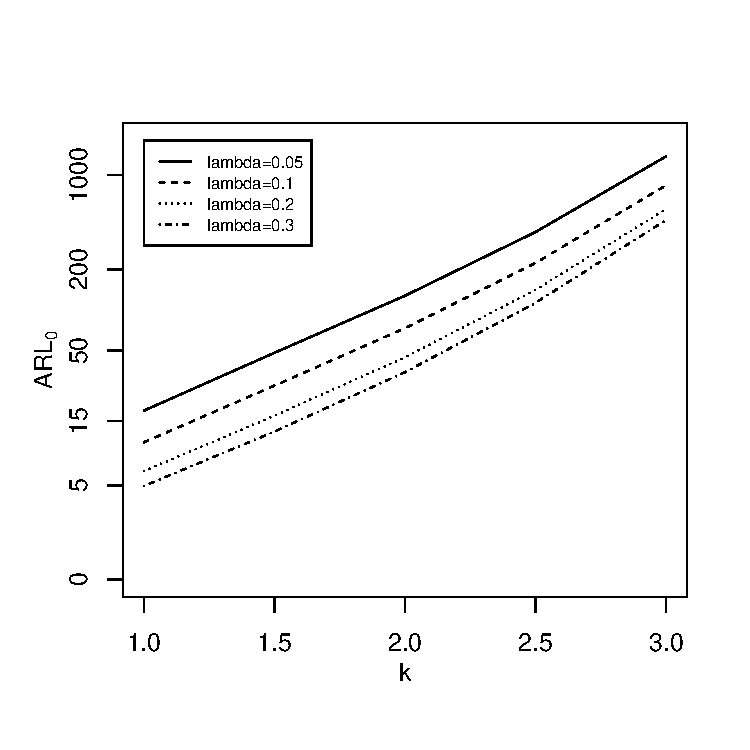
\includegraphics[height=0.3\textheight]{art/fig53}
\caption[$ARL_0$ for EWMA]{$ARL_0$ for EWMA. \newline Code from \url{http://users.phhp.ufl.edu/pqiu/research/book/spc/r-codes/fig53.r}}
\label{fig:arl_0_ewma}
\end{figure}

In the MA chart, we used the choice of $w$ to balance between quick response (small $w$) and sensitivity (large $w$).
EWMA has no window-width parameter, since it looks into all of history. On the other hand, we can control it by choosing $\lambda$. 
Large $\lambda$ gives more importance to the present. At the limit, $\lambda=1$, EWMA collapses to a standard Shewhart chart.



\subsection[CUSUM]{CUSUM Chart}
The \emph{cumulative sum} chart is similar to the EWMA in that it pools information from the history. 
The CUSUM simply sums all past deviations from the centre line.
If the process is in control, deviation will cancel each other, and their sum will vary around $0$. 
If the process is out of control, a drift will appear. 
The statistic to be plotted is 
\begin{align}
	C_t:= \sum_{j=0}^{t}(\bar{x}_j-\mu_0) = (\bar{x}_t-\mu_0) + C_{t-1}.
\end{align} 
Assuming $x_t \sim \gauss{\mu, \sigmabar^2}$ then if under control then $C_t \sim \gauss{\mu_0, t \sigmabar^2}$, we could thus set 
\begin{align}
\label{eq:cusum_simple_limits}
\begin{split}
	UCL &:= \mu_0 + \arm \sigma_{C_t}= \mu_0 + \arm \, \sqrt{t \sigmabar^2},  \\
	LCL &:= \mu_0 - \arm \sigma_{C_t}= \mu_0 - \arm \, \sqrt{t \sigmabar^2},
\end{split}
\end{align}
and $\arm=3$ as usual. 
You may encounter these limits in your favourite software (\rcode{qcc} package in \R), but it less often discussed in the literature. \cite{montgomery_introduction_2007} for example discuses very different limits. The discrepancy is explained in the following Extra Info. 

\begin{extra}
CUSUMs were introduced by \cite{page_continuous_1954}. 
\cite{montgomery_introduction_2007} adopts \citeauthor{page_continuous_1954}'s view and presents limits in two forms: the \emph{decision interval} (DI) form, \aka the \emph{tabular} form, and the graphical form known as a \emph{V-mask}.\marginnote{V-Mask}
These two control limits are equivalent. 
The fundamental difference between the control limits of \cite{page_continuous_1954}, and the ones presented until now, is that \citeauthor{page_continuous_1954} designed limits for the particular history of each process, while the limits until now, including Eq.(\ref{eq:cusum_simple_limits}) do not adapt to the particular history of the process.
As such, \citeauthor{page_continuous_1954}'s control limits are said to be \emph{adaptive}.\marginnote{Adaptive Contol Limits}
The limits in \cite{page_continuous_1954} are far from intuitive. 
This author has found \cite{ritov_decision_1990} to be the best explanation of \cite{page_continuous_1954}, but do not expect an easy reading...
\end{extra}









\section[Multivariate]{Multivariate Control Charts for Location}
\label{sec:multivariate}
% Wishart
% Srivastava Du
% PCA
% Higher criticism

\begin{example}[Intensive Care Unit]
\label{eg:intensive}
Consider an intensive care unit. 
The CTQs are the patient's blood pressure, temperature, etc.
We want to sound an alarm if the patient's condition deteriorates. 
Clearly, we can apply the univariate methodology above on each CTQ.
It is possible, that the deterioration is mild, so that it is not picked up by any CTQ individually (low power), but could have been noticed were we to aggregate signal over various CTQs. 
This is the concern of the current section. 
\end{example}


\subsection{Mass Univariate Control}
\label{sec:mass_univariate}

A first natural approach is to raise an alarm when \textbf{any} of the processes exceeds its respective control limits.
For $p$ independent processes, with univariate false alarm rate $\alpha^*$ each, then the joint false alarm rate is 
\begin{align}
	\alpha = 1-(1-\alpha^*)^p.
\end{align}
Clearly we could set $\alpha^*=1-\sqrt[p]{1-\alpha}$, so that the joint false alarm rate is under control, but we would not be enjoying the added sensitivity of pooling many CTQs together. 



\subsection[Hotteling's T2]{Hotteling's \tsq}
Hotteling's \tsq statistic is a generalization of the t-test due to \cite{hotelling_generalization_1931}.
To emphasize the relation to the t-test we write the classical t-statistic in the following weird form:
\begin{align}
	t^2(x_t)=n (\bar{x}_t-\mu_0) (\hat{\sigma_x}^2)^{-1} (\bar{x}_t-\mu_0).
\end{align}
This notation readily extends to the multivariate case. 
For $p$ CTQs, then $\bar{x}_t$ and $\mu_0$ are $p$-length vectors, and $\hat{\sigma}^2$ is replaced with the $p \times p$ covariance matrix $\hat{\Sigma}$.
Both $\mu_0$ and $\Sigma$ can be estimated from Phase I. 
\begin{definition}[Hotteling's \tsq statistic]
\begin{align}
\label{eq:hotteling}
	T^2(x_t) := n (\bar{x}_t-\hat{\mu}_0)' \hat{\Sigma}^{-1} (\bar{x}_t-\hat{\mu}_0).
\end{align}
\end{definition}
To derive the control limits, we will be assuming that $\x_{it}$ is $p$-variate Gaussian distributed, $\x_{it}\sim \gauss{\mu_0, \Sigma}$. 
Put differently, we assume that the $i$'th sample at period $t$ is a $p$-vector, such that its $j$'th coordinate $\x_{ijt}$ is univariate Gaussian, with mean $\mu_{0,j}$ variance $\Sigma_{j,j}$, and covariance with some other CTQ, $\x_{ij't}$, is given by $\cov{\x_{ijt},\x_{ij't}}=\Sigma_{j,j'}$. 

The sampling distribution of $T^2$ may depend on how $\mu_0$ and $\Sigma$ are estimated. 
For our purposes, where $\mu_0$ and $\Sigma$ are estimated in Phase I, we can safely use the following approximation
\begin{align}
	T^2 \overset{H_0}{\rightsquigarrow }\chi^2_p.
\end{align}
We can thus construct the control limit for this scenario:
\begin{align}
	UCL:= \chi^2_{1-\alpha,p}.
\end{align}

\begin{think}
Why is there no LCL? 
Think of a two-sided t-test \dots
\end{think}

Since the above limits have an (approximate) type-I error rate of $\alpha$, and the periods are independent, then we can readily apply Eq.(\ref{eq:arl_0}) to compute $ARL_0$.


\begin{remark}[Multivariate t or Multivariate Z?]
For simplicity, I do not distinguish between a t statistic and a Z statistic.
Since it is implied that variances are estimated in Phase I, then all t-statistics are actually Z statistics.
If variance were to be estimated in each period, then obviously my t-statistics would be proper t-statistics, and the reader should really consult  \cite[Ch.7]{qiu_introduction_2013} for details. 
\end{remark}




\subsection{Drill Down}
Your control chart just went outside the control limits and an alarm sounded.
The next natural question- what made the process go out of control?
In the univariate case, you should call your specialists team. 
In the multivariate case, there is another analysis stage you can/should do: \emph{drill down}.
By this we mean that we look an each of the $p$ processes separately to see which processes triggered the alarm.

The most natural way to drill-down, is to look at the raw univariate processes and see if any is out of the control limits.
Is it possible that a Hotelling alarm was sounded, but no single process seems out of control.
Absolutely! 
This was the whole point for which we used a multivariate control: because the signal is so mild that any single process had no power.

\begin{extra}[Many name to the drill-down]
In the electrical engineering literature, the ``drill down'' is also known as \emph{signal identification} that follows the initial \emph{signal detection}. 
In the analysis of variance literature (ANOVA) this is a \emph{post-hoc} test that follows an \emph{omnibus test}.
In the multiple testing literature, this is simply a multiple test. 
\end{extra}

\begin{extra}[Consonant tests]
As previously stated, it is possible that a multivariate alarm went off but no single variable seems out of control. 
This should not surprise you, since the whole motivation for doing the multivariate analysis was to draw power from several processes at the same time. 
The statistical literature does provide sets of multivariate and univariate tests that have to agree, meaning that it is impossible for the multivariate test to be rejected, without at least one univariate test to be rejected. 
This is known as \emph{consonant} tests. For more on that, the reader is referred to \cite{goeman_multiple_2011}.
\end{extra}







\section[Multivariate extensions]{Multivariate Control- Extensions}

Hotelling's \tsq is perhaps the first and most used multivariate test statistic.
Just like the univariate t-test, however, it is hardly the only multivariate test \dots





\subsection{Temporal Pooling of Multivariate Charts}
The basic problem: can we gain power by pooling multivariate data over several periods?
Sure!

\begin{definition}[Moving Sum Hotelling]
	The \emph{Moving Sum Hotelling} chart in a window of $w$ periods ending at $t$, is defined as
	\begin{align}
	M_t:= T^2(X_t)+\dots+T^2(X_{t-w+1})
	\end{align}
	where \tsq is Hotelling's test statistic $X_t$ is the matrix of $n$ samples on $p$ measurements at period $t$. 
\end{definition}
As before, we will typically, but not necessarily, use $\hat{\Sigma}$ from period I in \tsq. 

Since $T^2(X_t)$ is approximately $\chi^2_p$ distributed, periods are independent, and sums of Chi-square distributions are still Chi-square with the summed degrees of freedom\footnote{Trust me on this one.}, we have that for a process in control
\begin{align}
M_t \sim \chi^2_{wp}.
\end{align}
This readily suggests that the UCL for this chart is $\chi^2_{1-\alpha,wp}$. 

\begin{think}
	Is the moving sum Hotelling a Shewhart chart? 
	Can you design more multivariate charts with period pooling? 
	Can you derive their control limits?
\end{think}









\begin{example}[Vine Health]
\label{eg:irrigation}
Consider vine crops.
The crops are monitored for their health.
The health measurements (the CTQs) may be considerably affected by irrigation, weather, etc.
An unhealthy vine is thus one that behaves differently than the rest. 
The signal for out-of-control we seek is thus not in the mean CTQ of the vine, but rather in its correlation with others. 
We would like a multivariate version of the $s$ chart to monitor the health of our vines.  
\end{example}




\subsection[Multivariate s chart]{Multivariate $s^2$ Chart}
\label{sec:multivarite_s}

As discussed in the vine health example (Example \ref{eg:irrigation}), there are cases where the out-of-control behaviour is manifested in the covariance between CTQs, and not in their mean.
Recalling the Exploratory Data Analysis Section (\ref{sec:exploratory}), the most popular measure of multivariate relation is the \emph{covariance matrix}, $\hat{\Sigma}$ (Definition~\ref{def:covariance}).
To monitor changes in the correlations, we would like to compare the current covariance to its historic values, $\Sigma_0$. 
We would thus like to monitor $\hat{\Sigma}_t-\Sigma_0$, which is a $p\times p$ matrix. 
While we already know how to plot a matrix, plotting the evolution of a matrix in time, as is required for a control chart, is no simple task\footnote{Think about it. If a matrix is an image, then the evolution of a matrix in time is, well, simply a movie.}. 
Without going into the details of multivariate statistics, the fundamental idea is to summarize the matrix by a single number, so that it may be easily plotted, and control limits computed. 
We now provide several functions which can be thought of as \emph{norm} functions, i.e., functions that measure the ``distance'' from $\hat{\Sigma}_t$ to $\Sigma_0$. 




\begin{definition}[Frobenius norm]
The \emph{Frobenius norm} of matrix $A$, \aka the \emph{Hilbert-Schmidt norm}, or \emph{Schur norm} is defined as:
\begin{align}
	\normF{A}:= \sqrt{\sum_{ij} A_{ij}^2} 
\end{align}
As such, it merely treats the matrix as a stacked vector, and computes the Euclidean distance of the vector from zero.
\end{definition}
Using the Frobenius (matrix) norm for the process control, we would be plotting the time evolution of $\normF{\hat{\Sigma}_t-\Sigma_0}$.


\begin{definition}[Spectral norm]
Denoting the Euclidean distance of a vector $x$ from zero by $\norm{x}_{Euc}$, we can denote a matrix's \emph{spectral norm}, \aka \emph{operator norm}, or \emph{induced norm}, by: 
\begin{align}
	\norm{A}_{Spec} := \max_x \set{\norm{Ax}_{Euc}; \norm{x}_{Euc}=1}.
\end{align}
\end{definition}
The geometry of this definition is depicted in Figure~\ref{fig:operator_norm}.

\begin{figure}
\centering
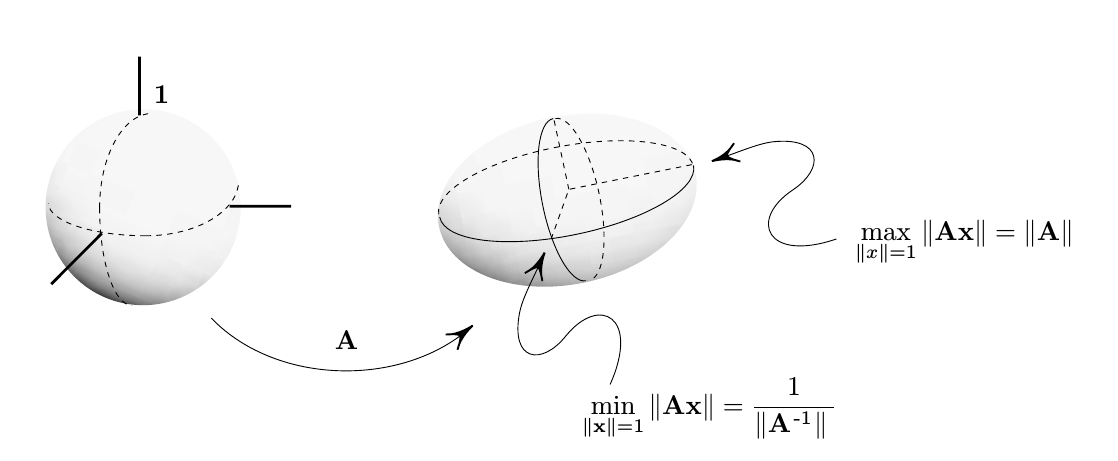
\includegraphics[width=0.7\linewidth]{art/operator_norm}
\caption[Geometry of Spectral Matrix Norms]{
\footnotesize
On the left: the unit circle in $\reals^3$. 
On the right: the ellipse is the image of the unit circle after transformed by matrix $A$. The operator norm is the distance between the origin and the furthest point on the ellipse. 
\newline Source: \cite{meyer_matrix_2001}.}
\label{fig:operator_norm}
\end{figure}

Using the Spectral (matrix) norm for the process control, we would be plotting the time evolution of $\norm{\hat{\Sigma}_t-\Sigma_0}_{Spec}$.


 
We will not present control limits for the generalized $s$ charts, but we do remind the reader that given a long enough Phase I, we can always look at the past values of the statistic for choosing the control limits. 




%\subsection[Mutivariate s chart]{Mutivariate $s$ chart}
%\label{sec:multivarite_s}
%
%As discussed in the vine health example (Example \ref{eg:irrigation}), there are cases where the out-of-control behaviour is manifested in the covariance between CTQs, and not in their mean.
%Recalling the Exploratory Data Analysis Section (\ref{sec:exploratory}), the most popular measure of multivariate relation is the \emph{covariance matrix} (Definition~\ref{def:covariance}).
%While we already know how to plot a matrix, plotting the evolution of a matrix in time, as is required for a control chart, is no simple task\footnote{Think about it. If a matrix is an image, then the evolution of a matrix in time is, well, simply a movie.}. 
%Without going into the details of multivariate statistics, the fundamental idea is to summarize the matrix by a single number, so that it may be easily plotted, and control limits computed. 
%To do so, we recall that in vector spaces, a function measuring the distance of a vector from the origin is named a \emph{norm function}.
%This idea may be generalized to matrix spaces. 
%By using the distance of a covariance matrix from a zero matrix (the origin), the covariance can be summarized into a single number. This distance function, is known as a \emph{matrix norm}.
%
%\begin{definition}[Operator $p$-norm]
%Operator $p$-norms are a class of matrix norms that view the matrix as the linear function it represents, so that the distance of a matrix from the origin is captured by the displacement this linear function causes upon its (normalized) inputs.
%Because it is induced by a vector norm, it is also known as an \emph{induced norm}.\marginnote{Induced norm}
%This also implies that there are as many matrix $p$-norms as there are vector $p$-norms. 
%To define the \emph{matrix} $p$-norm, we need to recall the $p$-norm of a vector $a$, which generalizes the idea of Euclidean distances:
%\begin{align}
%	\norm{a}_p:= \left( \sum_j |a_j|^p \right)^{1/p}
%\end{align}
%You may verify that setting $p=2$, you recover the standard Euclidean norm.
%Using vector $p$-norms, we can define the matrix $p$-norm 
%\begin{align}
%	\norm{A}_p:= \sup_x \set{\norm{Ax}_p; \norm{x}_p=1}.
%\end{align}
%\end{definition}
%
%
%\begin{figure}
%\centering
%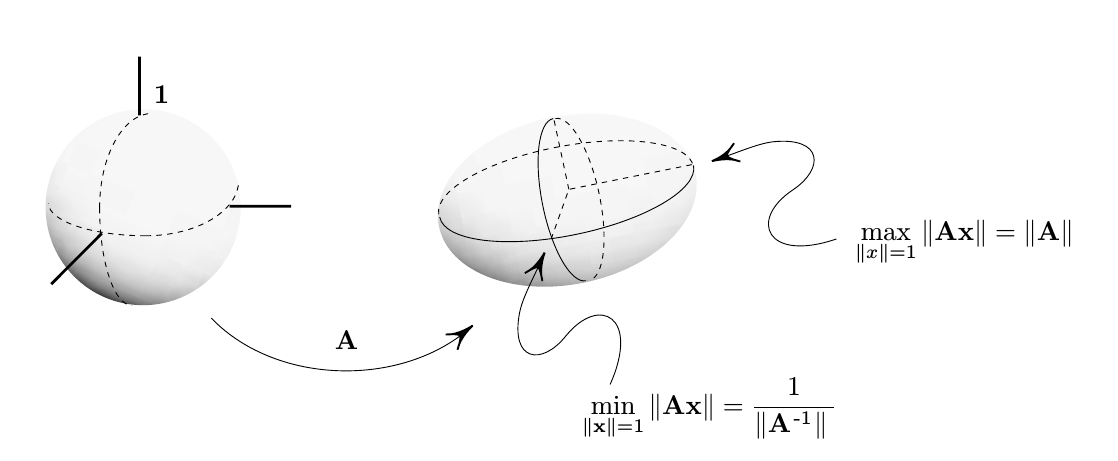
\includegraphics[width=0.7\linewidth]{art/operator_norm}
%\caption{
%\footnotesize
%On the left: the unit circle in $\reals^3$. 
%On the right: the ellipse is the image of the unit circle after transformed by matrix $A$. The operator norm is the distance between the origin and the furthest point on the ellipse. 
%\newline Source: \cite{meyer_matrix_2001}.}
%\label{fig:operator_norm}
%\end{figure}
%
%The various matrix operator norms, differ in the vector norm inducing them.
%The most popular, is by far the matrix $2$-norm, \aka the \emph{spectral norm}.
%Figure~\ref{fig:operator_norm} depicts the spectral norm of a matrix operating on $\reals^3$. 
%
%\begin{definition}[Spectral norm]
%The matrix $2$-norm, more commonly known as the \emph{spectral norm}, is merely the operator norm induced by the Euclidean vector norm, i.e., when $p=2$ . \marginnote{Spectral Norm}
%\begin{align}
%	\norm{A}_2:= \sup_x \set{\norm{Ax}_2; \norm{x}_2=1}	= \sqrt{\lambda_{max}(A'A)} = \sigma_{max}(A)
%\end{align}
%where $\lambda_{max}$ is the maximal eigenvalue, and $\sigma_{max}$ is the maximal singular value. 
%\end{definition}
%
%
%
%\begin{definition}[Frobenius (matrix) norm]
%The \emph{Frobenius norm}, \aka the \emph{Hilbert-Schmidt norm}, or \emph{Schur norm}, views the matrix as a square of numbers and is defined as follows:
%\begin{align}
%	\normF{A}:= \sqrt{\sum_{ij} a_{ij}^2} = \sqrt{\Tr(A'A)} = \sqrt{\sum \sigma_{j}(A)}
%\end{align}
%As such, it can be seen as a \emph{vector} $2$-norm, that stacks the matrix into a single vector, thus ignoring the fact that a matrix actually represents a linear function. 
%\end{definition}
%
%Equipped with any matrix norm, we may now generalize the $s$-chart by plotting the evolution of the (norm of the) covariance matrix and inspecting it for anomalies. 
%We will not discuss the theory required for setting the control limits, but we do remind the reader that given a long enough Phase I, we can always look at the history for choosing the control limits. 



\begin{extra}[Matrices and graphs]
Since a matrix defines a \emph{weighted graph} (and vise-versa), \aka a \emph{network}, any network similarity measure can be used to measure the distances between matrices, and can thus be used to summarize the covariance matrix and plot in a control chart.
\end{extra}







%\subsection{High-Dimensional Control Charts}
%
%\emph{High dimension} does not mean that $p$ is very large but rather the it is larger then $n$, or $\tau$. 
%To fix ideas, imagine that in the intensive care unit of Example~\ref{eg:intensive}, in each of $n=10$ measurements per day, we take $p=100$ different measurements such as pulse, temperature, etc.
%
%
%The problem in high-dimension is that we cannot properly estimate the covariance. 
%The fundamental idea to deal with the high-dimension is, well, to ignore the covariance when computing the statistic (but certainly not when computing the control limits!). 
%
%Two matters need to be considered when doing so:
%Is the type I error rate conserved?
%Is power lost?
%The answer to the first is- yes, if properly adjusting the control limits. 
%The answer to the second is- yes, but hopefully not too much.
%
%\begin{think}
%How many free parameters are in the covariance matrix of $p$ measurements?
%How many observations we would thus need to estimate this covariance?
%\end{think} 
%
%
%
%An example of a ``covariance ignoring'' test statistic, adapted from \cite{srivastava_test_2008}, is the following \footnote{I have simplified the actual statistic, so the reader is enouraged to read the reference before using the statistic.}:
%\begin{definition}[Simplified Srivastava-Du Statistic]
%\begin{align}
%\label{eq:srivastava_du}
%	 	T^{SD}(x) := n (\bar{x}-\mu_0)' D^{-1} (\bar{x}-\mu_0),
%\end{align}
%where $D$ is $\hat{\Sigma}$ with zeroes in all off-diagonal entries. 
%\end{definition}
%From Eq.(\ref{eq:srivastava_du}) we see that $T^{SD}$ is the same as Hotellig's \tsq in Eq.(\ref{eq:hotteling}) after forcing independence between coordinates.
%Changing from matrix notation to sum notation, we see that 
%\begin{align}
%	 	T^{SD}(x) = n \sum_{j=1}^p (\bar{x}_j - \mu_{0,j})^2 D^{-1}_{jj} .
%\end{align}
%But wait! 
%$D^{-1}_{jj}=(\Sigma_{jj})^{-1}$ is just the inverse variance of the $j$'th coordinate: $\frac{1}{Var(x_{1j},\dots,x_{nj})}$.
%This is rather good news, since it means that Eq.(\ref{eq:srivastava_du}) is nothing but the sum of the squared \textbf{univariate} t-statistics over the $p$ coordinates:
%\begin{align}
%	 	T^{SD}(x) =  \sum_{j=1}^p \frac{(\bar{x}_j - \mu_{0,j})^2}{\var{\bar{x}_j}}  .
%\end{align}
%
%We now see that a way to deal with the high-dimension, is to pool together $p$ univariate tests.
%Denoting the z-statistic of the $j$'th coordinate by $z_j:= \frac{(\bar{x}_j - \mu_{0,j})^2}{\var{\bar{x}_j}}$ we see that 
%$T^{SD}(x)= \normII{z_1,\dots,z_p}^2$, and that we can easily design new high dimensional test statistics in the form of
%\begin{align}
%\label{eq:marginal_test}
%	 	T(x) :=  f(z_1,\dots,z_p) .
%\end{align}
%where $f$ is some function measuring distance from the $\mu_0$ vector.
%
%
%\begin{think}
%Can you sugges other $f(z_1,\dots,z_p)$ functions that can make good signal detectors?
%\end{think}
%
%
%
%\begin{extra}[Inverting the covariance]
%Why do we need more observations than coordinates to invert $\Sigma$? 
%This is actually not a statistical matter but rather a linear algebra matter.
%If $dim(X)=n \times p$, and $n<p$, then rows of $X$ span a $n$ dimensional subspace of $\reals^p$. 
%With no loss of generality assume that $X$ is centred so that it has zero means. 
%In which case $\hat{Sigma}=X'X$, which is simply the Gram matrix. 
%Using the properties of Gram matrices, it follows that $\hat{Sigma}$ will not be invertible. 
%This ends the linear algebra. A more troubling fact is that even if algebraically possible to compute \tsq, it requires estimating so many parameters, that it will have poor statistical performance \citep{bai_effect_1996} which is exactly the high-dimension problem. 
%\end{extra}


%
%\subsection{Sparse Signals}
%
%We have already claimed that if signal exists only in a small subset of coordinates, i.e., it is \emph{sparse}, we can do better than \tsq, at least in the sense of power.
%The way to design test statistics for sparse signals, relies on the idea of computing coordinate-wise tests, and pooling them together, as in Eq.(\ref{eq:marginal_test}). 
%The mass-univariate test and chart (Section~\ref{sec:mass_univariate}) is an example of an alternative to \tsq if the signal is sparse. 
%It is constructed using 
%$f(z_1,\dots,z_p)=\max\set{z_1,\dots,z_p}$.
%
%
%\begin{think}
%Can you suggest other $f(z_1,\dots,z_p)$ functions that can make good signal detectors, if you assume the signal is ``hiding'' only in a small subset of coordinates?
%\end{think}
















\section{Economical Design of Control Charts}
\label{sec:economical_considerations}

Up until now, our design of control charts was driven by type-I error rates, and ARLs. 
Economical consideration were merely implied.
In this section, economical consideration take the driver's seat. 
We present a toy model, to demonstrate the economical optimization of design parameters in a \barxChart. 
Before beginning, a few remarks are in order. 

\begin{remark}[Economical Design of Control Charts]
\noindent
\begin{enumerate}
\item According to \cite{montgomery_introduction_2007} 
\begin{quote}
Saniga and Shirland (1977) and Chiu and Wetherill (1975) report that \textbf{very few practitioners} have implemented economic models for the design of control charts.
\end{quote}
Hmmmm.. Have things changed since 1977?
\item A comprehensive theoretical analysis of the optimization of a quality control system may be found in \cite{girshick_bayes_1952}. Again, \cite{montgomery_introduction_2007} is skeptic:
\begin{quote}
The optimal control rules are difficult to derive, as they depend on the solution to complex integral equations. Consequently, \textbf{the model’s use in practice has been very limited}.
\end{quote}
\end{enumerate}
\end{remark}

In light of the above skepticism, and following the lines of \cite{duncan_economic_1956}, we aim at the modest goal of an economical optimal \barxChart. 
Our target function is optimizing the expected income per hour, with respect to the design parameters:
\begin{align}
\label{eq:optimal_design}
	\max_{n,\arm,h}\set{\expect{C/T}}
\end{align}
where $C$ is the income between two productions halts, i.e., a \emph{cycle};
$T$ is the cycle duration;
$n$ is the number of samples per period;
$\arm$ governs the control limits via $UCL:= \mu_0+ \arm \sigma_{\bar{x}}= \mu_0+ \arm \sigma_x / \sqrt{n}$;
$h$ is the hours between sample periods. 

The parameters governing the solution are:
\begin{description}
\item[Income$_0$ ] Net income per production cycle when in control. Denoted $V_0$.
\item[Income$_1$] Net income per production cycle when out of control, after accounting for recall, legal damages, etc. Denoted $V_1$.
\item[Fixed sample cost] Fixed cost of sampling. Denoted $a_1$. 
\item[Variable sample cost] Variable cost sampling. Denoted $a_2$.
\item[Cost of True Positive] The cost to investigate and find an assignable cause; $a_3$.
\item[Cost of False Positive] The cost to investigate a false alarm; $a'_3$.
\end{description}


\begin{think}
How will the optimal $n,L,h$ change if the parameters of the problems are changed?
If $V_1$ is increased?
If $a_3$ is decreased?
\end{think}

For the purpose of this course, we will content ourselves with the above informal sensitivity analysis.
For completeness, the precise optimization problem is given in the next Extra Info.

\begin{extra}
We now need to establish how $\expect{C/T}$ is related to $n,\arm,h$. Here is our set of assumptions and notation:
\begin{enumerate}
\item When in control (IC), production is centred on $\mu_0$, assumed known. 
\item When out of control (OC), $\mu_1=\mu_0 \pm k \sigma_x$. 
\item When OC, production may proceed (!). 
\item Search and repair costs are not part of $C$.
\item OCs occur as a Poisson process, with rate $\lambda$ events per hour. The expected time from a sampling to an OC events is thus 
\begin{align}
	\tau := \frac{1-(1+ \lambda h) e^{-\lambda h}}{\lambda(1-e^{-\lambda h})}.
\end{align} 
\item The power to detect an OC is 
\begin{align}
	\pi:= \Phi(-\arm-k/\sqrt{n})+ (1-\Phi(\arm-k/\sqrt{n})).
\end{align}
\item The false alarm rate
\begin{align}
	\alpha:= 2 \Phi(-\arm).
\end{align}
\item Because of the Poisson process assumption,  $\expect{C/T}=\expect{C}/\expect{T}$. 
\item The expected cycle length:
\begin{align}
	\expect{T}= \frac{1}{\lambda}+ \frac{h}{\pi}- \tau  + D.
\end{align}
where $\frac{1}{\lambda}$ is time IC;
$\frac{h}{\pi}- \tau$ is the time the process is OC until detection;
$D$ is a fixed time to identify the assignable cause. 
\item The expected income per cycle
\begin{align*}
	\expect{C}= V_0 \frac{1}{\lambda} + 
	V_1 \left(\frac{h}{\pi}- \tau  + D  \right) - 
	a_3 -
	\frac{a'_3 e^{-\lambda h}}{1-e^{-\lambda h}} -
	(a_1+a_2n)\frac{\expect{T}}{h}.
\end{align*}
\end{enumerate}

Given all the above, we may now plug Eq.(\ref{eq:optimal_design}) into our favourite numerical solver to find the optimal $h,\arm,n$.

[TODO: add timeline]

\end{extra}






\section{Bibliographic Notes}
The contents of this chapter is mostly derived from \cite{montgomery_introduction_2007}. 
For a more mathematically rigorous treatment of the topic see \cite{basseville_detection_1993}.
For an \R oriented exposition of the topic, see \cite{qiu_introduction_2013}.
A quick digest review may be found in \cite{natrella_nist/sematech_2010}.
For multivariate process control, see for example \cite{ge_multivariate_2012}. 
For a technical discussion of multivariate statistics see \cite{anderson_introduction_2003}. 
For linear algebra, in particular matrix norms, see \cite{meyer_matrix_2001}. 
For some recent advances on high-dimension multivariate tests see \cite{srivastava_testing_2013} and references therein.
An excellent(!) reference for many useful, and regrettably overlooked, statistical techniques, see \cite{wilcox_introduction_2005}.
